\chapter{Imposers }\label{chapter-1.-imposers}

\section{Cognates from related languages}

I rely on `inverted reconstruction' (\cite[512-516]{Hockett1958}, \cite[346]{Anttila1972})
also called
`reconstructing forward in time' \citep[97]{Watkins1962}
and 
`reconstruction from the top down' \citep[1]{Blust1972}, a method known to Trans-Himalayan linguistics  \citep[]{jacques.michaud11naish}, but still poorly known, as evinced by an anonymous referee's admonition that reconstruction ``proceeds from the bottom up''. 
In keeping with this method, I intentionally compare Tosu forms to cognates in distantly related languages. 

\paragraph{}Now that the lengthy presentation of Old Chinese and its
reconstruction is in place, attention turns to innovations that Old
Chinese reflects vis-à-vis the Trans-Himalayan proto-language. Because
of the ambiguous and indirect nature of information about the
pronunciation of Old Chinese it is not easy to draw a sharp line between
Old Chinese and forms of speech ancestral to it. The most clear cut
methodological approach is to conceptualize as Old Chinese only as much
as can be known without recourse to comparative data. The application of
this methodological principle means that some of the mergers which
Baxter \& Sagart treat as taking place within the history of Chinese are
presented here (cf. §§-).

All of the changes from Trans-Himalayan to Chinese are mergers and these
changes do not interact with one another. As a consequence it is not
possible to resolve the relative chronology of these changes. The
approach here it to first present those mergers that Baxter \& Sagart
treat as Chinese internal and then turn to changes proposed entirely on
the basis of comparison to Tibetan and Burmese.

\paragraph{Merger of velars and dentals after
-i-.} In Old Chinese it is difficult to distinguish dentals
and velars after the vowel -i- (Baxter 1992: 435-437). Because Burmese
merges dentals and velars after -i-, it is of no help in resolving the
Chinese ambiguity (cf. §).

§a. Examples to be reconstructed *iŋ:

\begin{description}
\item
Chi. 年 \emph{nen} \textless{} *C.n{\sil{ˤ}}i{[}ŋ] (32-28a) `harvest, year',
Tib. {\tib{ན་ནིང་}} \emph{na-niṅ }'last year'
\item
Chi. 薪 \emph{sin} \textless{} *si[n] (32-33n) `firewood', Tib. {\tib{ཤིང་}} \emph{śiṅ} `wood'

\item
Chi. 莘 \emph{srin} \textless{} *sri[n] (32-33h) `long, drawn-out',
Tib. {\tib{རིང་}} \emph{riṅ} `long'

\item
Chi. 仁  \emph{nyin} \textless{} *ni{[}ŋ] (32-28f) `kindness', Tib.{\tib{སྙིང་}} \emph{sñiṅ} `heart'
\end{description}

§b. Examples to be reconstructed *-in:

\begin{description} \item
Chi. 憐 \emph{len} \textless{} *r{\sil{ˤ}}iŋ (32-26l) `love, pity', Tib. {\tib{དྲིན་
}} \emph{drin }'kindness'
\end{description}

\begin{description} \item
Chi. 辛 \emph{sin} \textless{} *sin (32-33a) `pungent, painful', Tib. {\tib{མཆིན་}} \emph{mčhin} `liver'
\end{description}

§c. Examples to be reconstructed *ik

\begin{description} \item
Chi. 縊 \emph{'ejH} \textless{} {\sil{*qˤ}}iks (08-05g) `strangle', Tib. {\tib{འཁྱིག་}} \emph{ḫkhyig}

\item
Chi. 節 \emph{tset} \textless{} *ts{\sil{ˤ}}ik (29-30e) `joint of bamboo', Tib. {\tib{ཚིགས་}} \emph{tshigs} `joint'

\item
Chi. 蝨 \emph{srit} \textless{} *sri{[}k] (29-35a) `louse', Tib. {\tib{ཤིག་}} \emph{śig}
\end{description}

\paragraph{Labial neutralization}. Because of
an early neutralization of labial and non-labial vowels before labial
consonants in Old Chinese, it is difficult to distinguish among *-up,
*-op, *-əp or among *-um, *-om, and *-əm (Baxter 1992: 541-553, 
\cite[306]{Baxter2014OldChinese}). In principle, comparative evidence is available to
support the reconstruction of one vowel or another.

\begin{description} \item
Chi. 入 \emph{nyip} \textless{} *nup (37-16a) `enter', Tib. {\tib{ནུབ་}} \emph{nub} `sink, set'

\item
Chi. 立 \emph{lip} \textless{} *k.rəp (37-15a) `stand (v.)', Tib. {\tib{འཁྲབ་
}} \emph{ḫkhrab} \textless{} *ḫkrəp `strike, stamp, tread heavily', OBur. {\burm{ရျပ်}} \emph{ryap} `stand, stop, halt'

\item
Chi. 三 \emph{sam} \textless{} *srum (38-30a) `three', Tib. {\tib{གསུམ་}} \emph{gsum}, Bur. {\burm{သုံး}} \emph{suṃḥ}

\item
Chi. 含 \emph{hom} \textless{} *Cə-m-{\sil{kˤ}}əm (38-03l') `hold in the mouth',
Tib. {\tib{འགམ}}་ \emph{ḫgam} \textless{} *ḫgəm `put in the mouth'

\item
Chi. 尋 \emph{zim} \textless{}*sə-l{[}ə]m (38-17) `warm up (food)',
Bur. {\burm{လုံ}} \emph{luṃ} `warm'
\end{description}

\paragraph{Inability to distinguish *-u- and
in -ə- before acutes.} In many cases Chinese
has the vowel *-ə where one expects *-u-. Because in Old
Chinese it is difficult to distinguish *‑ən, *‑ər, and *‑əj
from *‑un, *‑ur, and *‑uj (Baxter 1992: 427-428, 550; Hill 2012 `six
vowels' : 18-21), it is likely that this complication is due to an
incorrect reconstruction of the vowels in Old Chinese. 

\begin{description} \item
Chi. 運 \emph{hjunH} \textless{} *{\sil{[ɢ]ʷ}}ər-s 
(23-13d) `move', Tib. {\tib{འགུལ་}} \emph{ḫgul}
`move'
\item
Chi. 眉 \emph{mij} \textless{} *mrər 
(27-14a)
'eyebrow', WBur. {\burm{မွေး}} \emph{mweḥ} 
`body hair'
\item
Chi. 根 \emph{kon} \textless{} *[k]{\sil{ˤ}}ə[n] 
(33-01b) `root, trunk', Tib. {\tib{ཁུལ་མ་}} \emph{khul-ma}
`bottom or side of sth'
\item
Chi. 銀 \emph{ngin} \textless{} *ŋrə[n]
(33-01k) `silver,' Tib. {\tib{དངུལ་}} \emph{dṅul}
`silver', OBur. {\burm{ငုယ်}} \emph{ṅuy}
`silver'
\item
Chi. 齦 \emph{ng{\sil{jɨ}}n} \textless{} *ŋə[n] 
(33-01-) `gums', Tib. {\tib{རྙིལ་}} \emph{rñil}
`gums'
\item
Chi. 分 \emph{pjun} \textless{} *pə[n] 
(33-30a) `divide', Tib. {\tib{འབུལ་}} \emph{ḫbul},
{\tib{འཕུལ་}} \emph{ḫphul} `give'
\item
Chi. 塵 \emph{drin} \textless{} *[d]rə[n] 
(33-17a) `dust', Tib. {\tib{རྡུལ་}} \emph{rdul}  `dust'
\item
Chi. 貧 \emph{bin} \textless{} *(Cə.){[}b]rə[n]
(33-30v) `poor', Tib. {\tib{དབུལ་}} \emph{dbul}
\item
Chi. 軍 \emph{kjun} \textless{}
*[k]{\sil{ʷ}}ər 
(34-13a) `army', Tib.
 {\tib{གཡུལ་}} \emph{\textbf{g.yul}}
'army, battle'
\end{description}


\paragraph{Where and when to reconstruct *r}

\subparagraph{Inability to recognize -r- in
certain circumstances.} A wide variety of sound changes in the
history of the Chinese language lead to a merger of syllables with and
without medial *-r-. Thus, in many circumstance it is difficult to know
whether Old Chinese has a medial *-r-. Using `K' for velars, uvulars,
labio-velars, and labio-uvulars, `P' for labials, and `C' for any
consonants, the specific environments in which medial *-r- is lost
without trace are *K(r)ə, *K(r)u, *K(r)ək, *K(r)uk, *K(r)oŋ, *P(r)u,
*P(r)uk, *P(r)a, *Praj, *P(r)aw, and *C(r)ok in type B syllables, as
well as *C{\sil{ˤ}}(r)o in type A syllables (Baxter \& Sagart 2014: 214, 218,
243, 245).

§a. Some comparisons suggest a lack of medial *-r- in Old Chinese.

\begin{description} \item
Chi. 極 \emph{gik} \textless{} *[g](r)ək (05-04e) `ridge of roof,
highest point, centre', Tib. {\tib{མཁའ་}} \emph{mkhaḫ} `sky'

\item
Chi. 後 \emph{huwX} \textless{} *{\sil{[ɢ]ˤ}}(r)oʔ (10-08a) `behind', Tib. {\tib{འོག་}} \emph{ḫog} `under'

\item
Chi. 舅 \emph{gjuwX} \textless{} *[g](r)uʔ (04-16b) `maternal
uncle', Tib. {\tib{ཁུ་}} \emph{khu} `paternal uncle'

\item
Chi. 蜂�� \emph{phjowng} \textless{} *p{\sil{ʰ}}(r)oŋ (12-25st) `bee', Tib. {\tib{བུང་བ་}}
\emph{buṅ-ba}
\end{description}

§b. Other comparisons appear to confirm the presence of a medial *-r- in
Old Chinese.

\begin{description} \item
Chi. 蚼 \emph{xuwX} \textless{}{\sil{*qʰ}}{\sil{ˤ}}(r)oʔ (10-01n) `ant', Tib. {\tib{གྲོག་མོ་
}} \emph{grog-mo}

\item
Chi. 羽 \emph{hjuX} \textless{} *{\sil{ɢʷ}}(r)aʔ (01-24a) `feather', Tib. {\tib{སྒྲོ་
}} \emph{sgro} \textless{} *sg{\sil{ʷ}}ra

\item
Chi. 詖 \emph{pje} \textless{} *p(r)aj (18-16h) `one-sided, insincere
words', Tib. {\tib{ཕྲ་མོ་}} \emph{phra-mo} `slander'

\item
Chi. 披 \emph{phje }\textless{} *p{\sil{ʰ}}(r)aj (18-16j) `divide', Tib. {\tib{འབྲལ་
}} \emph{ḫbral} `be separate, to part', Bur. {\burm{ပြား}} \emph{prāḥ} `be divided
into parts'
\end{description}


\subparagraph{Pulleyblank's conjecture, *Cr- \textless{} *RC-}.
Returning to the Tibetan correspondences of those Chinese words that
have an unexpected medial *-r- permits further contemplation of Jacques'
third option. In most cases Tibetan exhibits a complex onset with a {\tib{སྔོན་འཇུག་}} \emph{sṅon-ḥjug} or {\tib{མགོ་ཅན་}} \emph{mgo-can} consonant, i.e.
 \emph{s}-,  \emph{d},  \emph{l}-, or \emph{g}-. The overall pattern of
unexpected Chinese *-r- cor­re­sponding to Tibetan complex onsets
entitles one to speculate that Chinese had some `pre-initial' in these
words that conditioned the same effects in Middle Chinese as Old Chinese
*-r-. This speculation extends Coblin's conjecture to environments
beyond the dental stops. Because it is unlikely that specifically *r-
was the `pre-initial' in all of these words, it is more suitable to
reconstruct *R- as a convention to mean `an indeterminate initial of a
complex onset which bears the same effects as *-r-'. Particularly based
on the comparison of Tibetan {\tib{གསོད་}} \emph{gsod} `kill' with Chinese 殺
 \emph{sreat} \textless{} *srat (21-29d), Pulleyblank posits *ks- as an
origin of Middle Chinese 生 \emph{sr}- (1965: 206-207). Gong similarly
proposes *rsat as the origin of Chinese 殺 \emph{sreat} \textless{}
*srat (21-29d) (2002{[}2001]: 171).

\begin{description} \item
Chi. 殼  \emph{khaewk} \textless{} *[{\sil{kʰ}}]{\sil{ˤ}}rok \textless{}
*R{[}{\sil{kʰ}}]{\sil{ˤ}}ok (11-03a) `hollow shell, hollow', Tib. {\tib{སྐོག་}} \emph{skog}
'shell, peel'
\item
Chi. 銀  \emph{ngin} \textless{} *ŋrə[n] \textless{} *Rŋə[n]
(33-01k) `silver', Tib. {\tib{དངུལ་}} \emph{dṅul}
\item
Chi. 貧  \emph{bin} \textless{} *(Cə.){[}b]rə[n] \textless{}
*(Cə.)R{[}b]ə[n] (33-30v) `poor', Tib. {\tib{དབུལ་}} \emph{dbul}
\item
Chi. 虎  \emph{xuX} \textless{} {\sil{*qʰ}}{\sil{ˤ}}raʔ `tiger' \textless{} *R{\sil{qʰ}}{\sil{ˤ}}aʔ
(01-18b), 
Tib. 
%{\protect\[hypertarget{anchor-51}{}{}
Chi. 虎 \emph{xuX}
\textless{} {\sil{*qʰ}}{\sil{ˤ}}raʔ `tiger' \textless{} *R{\sil{qʰ}}{\sil{ˤ}}aʔ (01-18b), Tib. {\tib{སྟག་}} \emph{stag}
\item
Chi. 膚  \emph{pju} \textless{} *pra \textless{} *Rpa (01-51g) `skin',
Tib. {\tib{ལྤགས་}} \emph{lpags} (p. n. )
\item
Chi. 殺  \emph{sreat} \textless{} *srat \textless{} *Rsat (21-29d)
'kill', Tib. √sad (pres. {\tib{གསོད་}} \emph{gsod})
\item
Chi. 三  \emph{sam} \textless{} *srum \textless{} *Rsum (38-30a) `three',
Tib. {\tib{གསུམ་}} \emph{gsum}
\end{description}

§a. There are two comparisons, in which the Tibetan cognates have a
simplex onset; these are apparent counterexamples to Pulleyblank's
conjecture.

\begin{description} \item
Chi. 蝨  \emph{srit} \textless{} *sri{[}k] (29-35a) `louse', Tib. {\tib{ཤིག་}} \emph{śig}
\item Chi. 沙  \emph{srae} \textless{} *s{\sil{ˤ}}raj (18-15a) `sand', Tib. {\tib{ས་}} \emph{sa} `earth'
\end{description}

In the first of these apparent exceptions, the Japhug Rgyalrong cognate
 \emph{zrɯɣ} `louse' confirms the Chinese onset *sr- is original. One may
suggest that Tibetan underwent a change *sr- \textgreater{} ś-
conditioned by the vowel -i-. Because the change *sr- \textgreater{} ś-
preceded Dempsey's law *-eŋ \textgreater{} -\emph{iṅ} (cf. §), Tibetan {\tib{སྲིང་མོ་}} \emph{sriṅ-mo} \textless{} *sreṅ-mo `sister of a man' avoided
the former change (cf. Chi. 甥 \emph{sraeng} \textless{} *s.reŋ
{[}09-25g] `son-in-law'). I have no explanation for the correspondence
seen in `sand'.

§b. Fitting Burmese evidence into the overall picture of the sibilants
is not straightforward (cf. §).

\subparagraph{Coblin's conjecture, *Tr- \textless{} *rT-}. Coblin
proposes that the correspondence of Chinese *Tr with Tibetan Tr- be
reconstructed *rT in the proto-language (1986: 21-22). Gong reiterates
this suggestion, further conjecturing that *rT continued into the Old
Chinese period (2002{[}2000]: 171). Handel concurs with Gong that *Tr
should take the form *rT in Old Chinese (2009: 211-217); he offers the
Chinese internal evidence that `dimidiated clusters' suggest *Kr- (e.g.
康良 \emph{khang ljang} `empty' \textless{} *{\sil{kʰ}}r-) and *Pr- (e.g. 朦朧
 \emph{muwng luwng} `indistinct' \textless{} *mr{\sil{ˤ}}-) but not *tr- (2009:
215). Because this proposal improves cor­re­spon­dences to Tibetan, I
assume it as a working hypothesis. The orthographic representation of
Coblin's conjecture as a change from the proto-language to Old Chinese
via a metathesis, i.e. *rT- \textgreater{} *Tr- does not necessarily
have its face value. Instead, *‑r- in Baxter \& Sagart's system indexes
all origins of Middle Chinese retroflex initials (cf. §), division-ii
rimes (cf. §), and \emph{chóngniǔ} rank-iii rimes (cf. §), including
both medial *-r- and, if one accepts Coblin's conjecture, initial *r-,
at least before dentals. In other words, if Coblin's conjecture is
correct then the sequence *rT- existed as such in Old Chinese.

\begin{description} \item
Chi. 撞 \emph{draewng} \textless{} *[N-t]{\sil{ˤ}}roŋ \textless{}
*[N-]r{[}t]{\sil{ˤ}}oŋ (12-08f') `strike', Tib. {\tib{རྡུང་}} \emph{rduṅ}
\item
Chi. 塵 \emph{drin} \textless{} *[d]rə[n] \textless{}
*r{[}d]ə[n] (33-17a) `dust (n.)', Tib. {\tib{རྡུལ་}} \emph{rdul}
\item
Chi. 冢 \emph{trjowngX} \textless{} *[t]roŋʔ \textless{}
*r{[}t]oŋʔ (11-13h), `tomb mound', Tib. {\tib{རྡུང་}} \emph{rduṅ} `small
mound, hillock', WBur. {\burm{တောင်}} \emph{toṅ} \textless{} *tuṅ `hill,
mountain'
\item
Chi. 晝 \emph{trjuwH} \textless{} *truks \textless{} *rtuks (14-09a)
'time of daylight', Tib. {\tib{གདུགས་}} \emph{gdugs} `mid-day, noon'
\item
Chi. 綴 \emph{trjwet} \textless{} *trot \textless{} *rtot (22-10b)
'bind', Tib. √rtod (pres. {\tib{རྟོད་}}) `tether, fasten, secure'
\item
Chi. 椓 \emph{traewk} \textless{} *tr{\sil{ˤ}}ok \textless{} *rt{\sil{ˤ}}ok (11-13c)
'beat, strike', Tib. {\tib{རྡུག་}} \emph{rdug} `conquer'
\end{description}

§a. Coblin's conjecture still leaves many examples of medial *-r- in
Chinese without a corresponding rhotic in Tibetan or Burmese.

\begin{description} \item
Chi. 殼 \emph{khaewk} \textless{} *[{\sil{kʰ}}]{\sil{ˤ}}rok (11-03a) `hollow shell,
hollow', Tib. {\tib{སྐོག་}} \emph{skog} `shell, peel', WBur. {\burm{ခေါက်}} \emph{khok}
\textless{} *ˀkuk `bark (n.)', Atsi  \emph{ˀku⁵⁵}
\item
Chi. 銀 \emph{ngin} \textless{} *ŋrə[n] (33-01k) `silver,' Tib.{\tib{དངུལ་}} \emph{dṅul}, OBur. {\burm{ငုယ်}} \emph{ṅuy}
\item
Chi. 眉 \emph{mij} \textless{} *mrər (27-14a) `eyebrow', WBur. {\burm{မွေး}} \emph{mweḥ} \textless{} *muyḥ `body hair'
\item
Chi. 貧 \emph{bin} \textless{} *(Cə.){[}b]rə[n] (33-30v) `poor',
Tib. {\tib{དབུལ་}} \emph{dbul}
\item
Chi. 虎 \emph{xuX} \textless{} {\sil{*qʰ}}{\sil{ˤ}}raʔ `tiger' (01-18b), Tib.
\protect\hypertarget{anchor-49}{}{}Chi. 虎 \emph{xuX} \textless{}
{\sil{*qʰ}}{\sil{ˤ}}raʔ `tiger' (01-18b), Tib. {\tib{སྟག་}} \emph{stag}
\item
Chi. 膚 \emph{pju} \textless{} *pra (01-51g) `skin',\footnote{Perhaps
  cognate to the {\burm{
  ပြား}} \emph{prāḥ} (\textless{} *brāḥ) of WBur. {\burm{အရေပြား}} \emph{a-re-prāḥ} `skin' in which case the Tibetan form is potentially
  not cognate.} Tib. {\tib{ལྤགས་}} \emph{lpags}
\item
Chi. 蝨 \emph{srit} \textless{} *sri{[}k] (29-35a) `louse', Tib. {\tib{ཤིག་}} \emph{śig}
\item
Chi. 殺 \emph{sreat} \textless{} *srat (21-29d) `kill', Tib. √sad (pres. {\tib{གསོད་}} \emph{gsod}), Bur. {\burm{သတ်}} \emph{sat} \textless{} *ˀsat, Lashi
 \emph{ˀsa:tH}
 \item
Chi. 三 \emph{sam} \textless{} *srum (38-30a) `three', Tib. {\tib{གསུམ་}} \emph{gsum}, Bur. {\burm{သုံး}} \emph{suṃḥ} \textless{} *suṃḥ, Lashi  \emph{sɔmH}
\item
Chi. 沙 \emph{srae} \textless{} *s{\sil{ˤ}}raj (18-15a) `sand', Tib. {\tib{ས་}} \emph{sa} `earth', Bur. {\burm{သဲ}} \emph{sai} `sand'
\end{description}

\footnote{For a discussion of Handel's attempt to explain the correspondence of *sr- in
Chinese to Tibetan \emph{s}- (or \emph{ś}-) 
\citeyearpar[201-209]{Handel2009} and Jacques' 
\citeyearpar{jacques15sr}
rejection of his proposals see \citet[198-200]{hill2019phonology}.} 





\section{Early loans in and out of Chinese}


{Loan from Chinese}

\begin{itemize}
    \item {\Large{萬}} OChi. *t.mans `ten thousand'
    \item Old Turkic \textit{tümen} `ten thousand'
    \item Tocharian A \textit{tmān}; B \textit{tmane}, \textit{tumane} `ten thousand'
    \item 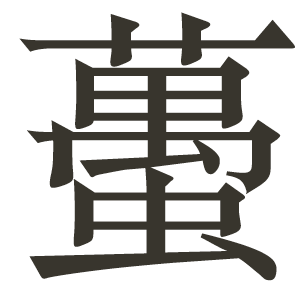
\includegraphics[scale=0.12]{Chapter1/chai2.png} MChi. \textit{trhaejH} <  OChi. *t.{\sil{m̥}}rats 
     `scorpion'
\end{itemize}




{Indo-Aryan loans into Old Chinese} 

\begin{itemize}
    \item {馬} 
    %{\emph{\sil{mǎ}}} < 
    MChi. {\emph{\sil{maeX}}} < OChi. *{\emph{\sil{rmˤaʔ}}}
    \\ from Indo-Aryan *{\emph{\sil{áru̯ant}}}-`steed, courser'   
    \item {車}  
    %{\emph{\sil{chē}}} < 
    MChi. {\emph{\sil{tsyhae}}} < OChi. *{\emph{\sil{təqʰra}}} `chariot'
    \\ from Indo-Aryan *{\emph{\sil{cakrá-}}} `chariot'
\end{itemize}


  

Archaeological support for Indo-Aryan speakers introducing the horse and chariot to China circa 1250 BCE. \\

%\vspace{1mm}
%N.B. This agrees with the findings of archaeology.




goose

horse

ten thousand in Tokharian

\section{Hàn dynasty Chinese transcriptions of Indic Buddhist terms}

\paragraph{} 
\label{origins-of-the-tones-and-final-clusters}
Early Chinese transcriptions of foreign words sometimes show the
departing tone cor­re­spond­ing to foreign -\emph{s} ().\footnote{The
  examples are from Pulleyblank (1962: 217-219); I provide the Han
  Chinese reconstructions for reference, based on Schuessler 2009. These
  first seven examples Pulleyblank collected from an article by Bailey
  (1946). The following three examples are from Lokakṣema's (支婁迦讖
  circa 147-189 CE) translation of the \emph{Prajñāpāramitā Sūtra}
  (\emph{Dào Xíng Bānruò Jīng} 道行般若經, T. 224, cited after
  Pulleyblank). The remaining examples come from early historical
  sources. The example of 劫貝 for Skt.  \emph{kārpāsa} `cotton' is from
  Schuessler (2009: 22). In the case of the Skt. examples one must keep
  in mind that the final -a in Sanskrit is likely to have already become
  mute before these words were brought to China. } 
  
\begin{figure}[t]
    \centering
\begin{tabular}{|llll|}
\hline
Character &
Middle Chinese &
Hàn Chinese &
Foreign language transcribed \\ \hline
波羅奈 &
pa la najH &
{\sil{pɑi lɑi nɑs}} & 
Skt. 
{\emph{vārāṇasī}} \\
三昧 &
sam mwojH &
{\sil{sɑm məs}} & 
Skt. {\emph{samādhi}} (Skt. dh- > Prakrit z-) \\
提謂 &
tej hjwɨjH &
{\sil{de wus}} &
Skt. {\emph{trapuṣa}}, Khot. {\emph{tträväysa}} \\
忉利 &
taw lijH &
{\sil{tɑu lis}} &
Skt. {\emph{trāyastriṃśa}}, Khot. {\emph{ttāvatrīśa}} \\
阿魏 &
'a ngjwɨjH &
{\sil{ʔɑ ŋuih}} & \makecell{
Khot. {\emph{aṃguṣḍä}}, Tokh. B: {\emph{ankwaṣ}}, \\ Uighur {\emph{'nk'pwš}} `asafoetida'} \\
舍衞 &
syaeX hjwejH &
{\sil{śaʔ was}} &
Skt. {\emph{śrāvastī}} \\
迦維羅衛 &
kae ywij la hjwejH &
{\sil{kai wi lɑi was}} & 
Skt. {\emph{kapilavastu}} \\
阿會亘 & 
'a hwajH hwan &
{\sil{ʔɑ ɣuɑs huar}} &
Skt. {\emph{abhāsvara}} \\
阿迦貮吒 &
'a kae nyijH traeH & 
{\sil{ʔɑ ka ńis ṭah}} &
Skt. {\emph{akaniṣṭha}} \\
首陀衛 &
syuwX da hjwejH &
{\sil{śuʔ dɑi was}} &
Skt. {\emph{śuddhāvāsa}} \\
對馬 &
twojH maeX &
{\sil{tuəs maʔ}} &
Jp. Tusima (modern Tsushima) \\
都賴 &
tu lajH &
{\sil{tɑ lɑs}} & 
Talas \\
罽賓 &
kjejH pjien &
{\sil{kɨɑs pin}} & 
Kashmir \\
蒲纇 &
bu lwojH &
{\sil{bɑ luis}} &
Mong. {\emph{bars}} `tiger'  \\
劫貝 &
kjaep pajH &
{\sil{kɨɑp pɑs}} &
Skt. {\emph{kārpāsa}} `cotton' \\ \hline
\end{tabular}
    \caption{the 去聲 qùshēng tone transcribing foreign -s}
    \label{fig:qusheng-as-s}
\end{figure}


Transcriptions of foreign words





{Falling tone -H from *-s}

\begin{tabular}{|l|l|l|l|}
\hline
Character &
MChi. &
Hàn Chi. &
Skt. \\ \hline
波羅奈  &
{\sil{pa la naj\textbf{H}}} &
{\sil{pɑi lɑi nɑ\textbf{s}}}  &
vārāṇa\textbf{s}ī \\
%三昧 &
%sam mwojH &
%sɑm məs  &
%Skt. samādhi \\
提謂 &
{\sil{tej hjwɨj\textbf{H}}} &
{\sil{de wu\textbf{s}}} &
trapuṣa
%, Khot. tträväysa 
\\
忉利 &
{\sil{taw lijH}} &
{\sil{tɑu li\textbf{s}}} &
trāyastriṃ\textbf{ś}a
%, Khot. ttāvatrīśa 
\\
%阿魏 &
%'a ngjwɨjH &
%ʔɑ ŋuih &
%Khot. aṃguṣḍä, Tokh. B: ankwaṣ, Uighur 'nk'pwš 'asafoetida' \\
舍衞 &
{\sil{syaeX hjwej\textbf{H}}}&
{\sil{śaʔ wa\textbf{s}}} &
śrāva\textbf{s}tī \\
迦維羅衛 &
{\sil{kae ywij la hjwej\textbf{H}}} &
{\sil{kai wi lɑi wa\textbf{s}}} & 
kapilavastu \\
阿會亘  &
{\sil{'a hwaj\textbf{H} hwan}} &
{\sil{ʔɑ ɣuɑ\textbf{s} huar}} &
abhā\textbf{s}vara \\
阿迦貮吒 &
{\sil{'a kae nyij\textbf{H} traeH}} & 
{\sil{ʔɑ ka ńi\textbf{s} ṭah}} &
akani\textbf{ṣ}ṭha \\
首陀衛  &
{\sil{syuwX da hjwej\textbf{H}}}  &
{\sil{śuʔ dɑi wa\textbf{s}}} &
śuddhāvā\textbf{s}a \\ \hline
\end{tabular}






{Transcriptions of foreign words}
烏弋山離 \textit{'u yik srean lje}
< *{\sil{ʔâ lək sran raj}}
'Alexandria' (36 BCE)

%亘 (Lokakṣema, 178-189 CE) 
%亘 sjwen (25-12a), Skt. ābhāsvara 阿會
%洹 hwan (25-12g), Skt. parinirvāṇa 般泥洹 %
%桓 hwan (25-12f), Skt. śakro devānām indra 釋提桓因 


\section{Rhyme tables}
\paragraph{}
The
rime tables of the 宋 Sòng dynasty provide the most important imposer for Middle Chinese. The most famous is the 韻鏡
 \emph{Yùnjìng} published by 張麟之 Zhāng Línzhī in 1161, but the 七音略
 \emph{Qīyīnlüè}, which appeared the same year in the 通志 \emph{Tōngzhì}
encyclopedia by 鄭樵 Zhèng Qiáo, is also influential. The
in­ter­pre­ta­tion of these sources is complex and con­tro­versial (cf. \cite{Branner2000c},
\cite[8-20]{Baxter2014OldChinese},
\cite{Handel2014},
\cite{jacques17traditional}).

\paragraph{The initials of the rime tables.}
The  \emph{Yùnjìng} explicitly distinguishes initials into place and
manner of articulation with terms such as labial (唇 \emph{chún}),
dental (舌 \emph{shé}), voiceless (清 \emph{qīng}), voiceless aspirated
(次清 \emph{cìqīng}), etc. the \emph{Qīyīnlüè} distinguishes 36 initials
by giving an example of each.\footnote{The preface to the  \emph{Yùnjìng}
  contains a list of the same list of 36 initials, but the body of the
  text does not classify characters according to these initials.} Thus,
what the  \emph{Yùnjìng} describes as a `voiceless labial' the
 \emph{Qīyīnlüè} refers to acrophonically as the 幫 \emph{p}(\emph{ang})
initial. 
Associating sounds with the 36 initials of the \emph{Qīyīnlüè} and the
articulatory categories of the \emph{Yùnjìng} is feasible. Hereafter I
refer to `the rime tables' when the distinction between the
 \emph{Yùnjìng} and the the \emph{Qīyīnlüè} is clear or unimportant.\footnote{Note that 30
  initials of the Dūnhuáng fragments (see note ) omit initial 娘
  \emph{nr-}. Initials 匣 \emph{h-} and 雲 \emph{hj-} (the latter a
  subset of the 喻 yù initial category of the rime tables) are
  also in complementary distribution.}



\section{Táng dynasty Tibetan transcriptions of Chinese}


\section{Sino-Xenic}
Although the modern Chinese dialects do not generally allow a
distinction to be drawn between  \emph{chóngniǔ} rank-iii readings and
 \emph{chóngniǔ} rank-iv readings,
in many cases Sino-Vietnamese character readings also provide evidence for
this distinction; 碑  \emph{pje} has the Sino-Vietnamese reading
 \emph{bi} whereas 卑 \emph{pjie} has the Sino-Vietnamese reading
 \emph{ti} 
 \citep[86]{Baxter1977}.

\section{Yuán dynasty ‘Phags-pa script transcriptions of Chinese}

Although the modern Chinese dialects do not generally allow a
distinction to be drawn between  \emph{chóngniǔ} rank-iii readings and
 \emph{chóngniǔ} rank-iv readings,
in many cases the Ḥphags-pa script transcriptions of these characters in
the 14th century 蒙古字韻  \emph{Měnggǔ zìyùn} distinguishes
 \emph{chóngniǔ} rank-iii and \emph{chóngniǔ} rank-iv (\cite[]{Shen2005chongniu}); in this source 碑  \emph{pje} is transcribed
 
\includegraphics[width=0.25cm]{Chapter5/Phagspabue.png}
\textless{}bue\textgreater{} and 卑 \emph{pjie} is transcribed as
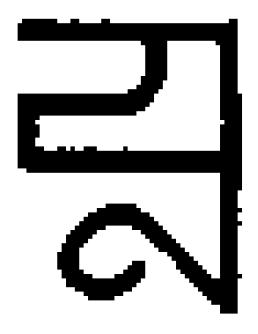
\includegraphics[width=0.25cm]{Chapter5/PhagspaBi.png}
\textless{}bi\textgreater{} (\cite[167]{Shen2005chongniu},
\cite[122 and 126]{Coblin2007}). 


